% !TeX root = ../../thesis.tex
\chapter{Advanced model with kinetics}\label{ch:kinetics}


\begin{shaded}
This chapter is based on prepared manuscript to be submitted to  \textit{npj Computational Materials}:\\
M. Barzegari, C. Wang, S.V. Lamaka, G. Zavodszky, and L. Geris, ``Interface-coupled multiphysics computational modeling of local pH changes during the biodegradation of magnesium biomaterials,'' will be submitted to \textit{npj Computational Materials}.
\end{shaded}

\section{Introduction}

The biodegradation behavior of Mg is investigated in corrosion tests, in which the selection of the corrosive media plays an important role since it affects the underlying chemical reactions \cite{Mei2020}. By considering the main application of the biomaterial, which can be tissue engineering scaffolds, vascular stents, or orthopedic fixation implants, the corrosive media can be selected to be a representative of the service environment. The most basic form of the medium is a saline (NaCl) solution, in which the degradation rate is the highest possible \cite{Mei2020}. More complex solutions can be used to mimic the behavior of body environment by taking into account more body fluid components, the most popular of which are the Ringer's solution, PBS (phosphate buffered saline), SBFs (simulated body fluids), HBSS (Hank's balanced salt solution), and Earle's balanced salt solution (EBSS) \cite{Mei2020}. Adding more organic components to the solution will make it ready to simulate cell culture conditions. The common media for this purpose are MEM (Minimum Essential medium) and DMEM (Dulbecco's modified Eagle's medium) \cite{Mei2020}. 

A wide range of various studies have already investigated the effect of different components in the aforementioned corrosive media on the degradation behavior of Mg materials \cite{Mei2019,Zeng2014,Johnston2017, Lamaka2018,Mei2019a}. A typical composition of "simulated body fluid" solutions (such as SBF, HBSS, and EBSS) is chloride, carbonate, phosphates, sulfate, and calcium. The individual effect of these components on the rate of degradation of Mg has been extensively studied, in which it has been observed that carbonate and phosphate slow down the rate while the effect of sulfate is negligible \cite{Johnston2017,Mei2019a}. The concentration of $\mathrm{HCO}_{3}^{-}$ affects the pH buffering capacity and the degradation rate of Mg simultaneously \cite{Xin2011}.

The effect of calcium ion is more complex because it has been found that $\mathrm{Ca}^{2+}$ doesn't contribute to the Mg corrosion directly \cite{Willumeit-Roemer2019}, but a mixed effect of $\mathrm{Ca}^{2+}$, $\mathrm{Mg}^{2+}$, $\mathrm{HCO}_{3}^{-}$, and $\mathrm{H}_{2} \mathrm{PO}_{4}^{-} / \mathrm{HPO}_{4}^{2-}$ forms a co-precipitation layer on the corroded surface of Mg, slowing down the corrosion rate of commercially pure Mg as well as some the of the Mg alloys \cite{Mei2019,Lamaka2018}. It has been also reported that although various Mg alloys show different intrinsic degradation behavior in NaCl solution, they possibly behave similarly in simulated body fluids \cite{Agha2016,Mei2019a}. Since the humoral regulations inside the human body control the changes in pH of body fluids, it's common to use pH buffers to mimic a similar condition, but it should be taken into account that buffering solution may affect the degradation rate of Mg \cite{Cui2017,Kannan2017}. pH buffers may also delay the formation of the precipitate layer \cite{Lamaka2018}. An alternative solution to address this issue is to use natural pH buffers such as $\mathrm{HCO}_{3}^{-}/\mathrm{CO}_{2}$, a technique that is commonly used for immersion tests under cell culture conditions. In this situation, an equilibrium between $\mathrm{H}_{2} \mathrm{CO}_{3}\left(\mathrm{CO}_{2}\right)$, $\mathrm{HCO}_{3}{ }^{-}$, and $\mathrm{CO}_{3}{ }^{2-}$ keeps the pH constant. As a result, using simulated body fluids for corrosion tests without additional synthetic pH buffer is still acceptable \cite{Lamaka2018,Mei2019a}.

The major reactions occurring in simulated body fluids can be written as:
\begin{equation}
\mathrm{Mg}+2 \mathrm{H}_{2} \mathrm{O} \rightarrow \mathrm{Mg}(\mathrm{OH})_{2}+\mathrm{H}_{2} 
\end{equation}
\begin{equation}
2 \mathrm{Mg}+2 \mathrm{H}_{2} \mathrm{O}+\mathrm{O}_{2} \rightarrow 2 \mathrm{Mg}(\mathrm{OH})_{2}
\end{equation}
\begin{equation}
5 \mathrm{Ca}^{2+}+3 \mathrm{PO}_{4}^{3-}+\mathrm{OH}^{-} \rightarrow \mathrm{Ca}_{5}\left(\mathrm{PO}_{4}\right)_{3} \mathrm{OH}
\end{equation}
\begin{equation}
\mathrm{Ca}^{2+}+2 \mathrm{OH}^{-} \rightarrow \mathrm{Ca}(\mathrm{OH})_{2}
\end{equation}
\begin{equation}
\mathrm{Mg}^{2+}+\mathrm{CO}_{3}^{2-} \rightarrow \mathrm{MgCO}_{3}
\end{equation}
\begin{equation}
\mathrm{Ca}^{2+}+\mathrm{CO}_{3}^{2-} \rightarrow \mathrm{CaCO}_{3}
\end{equation}
\begin{equation}
 3 \mathrm{Mg}^{2+}+2 \mathrm{PO}_{4}^{3-} \rightarrow \mathrm{Mg}_{3}\left(\mathrm{PO}_{4}\right)_{2}
\end{equation}
\begin{equation}
\mathrm{CO}_{3}^{2-}(a q)+H^{+}(a q) \rightarrow \mathrm{HCO}_{3}^{-}(a q)
\end{equation}
\begin{equation}
P O_{4}^{3-}(a q)+H^{+}(a q)\rightarrow \mathrm{HPO}_{4}^{2-}(a q)
\end{equation}

Then, the aforementioned protection layer is formed on the corroded surface as a hydroxyapatite-like precipitation according the following reaction \cite{Atrens2015,Song2009,Silva2018,Jiang2019}:
\begin{equation}
\begin{aligned}
m \mathrm{Mg}^{2+}+n \mathrm{Ca}^{2+}&+x \mathrm{H}_{2} \mathrm{PO}_{4}^{-} / \mathrm{HPO}_{4}^{2-}+y \mathrm{HCO}_{3}^{-}+z \mathrm{OH}^{-}\\
& \rightarrow \mathrm{Mg}_{m} \mathrm{Ca}_{n}\left(\mathrm{PO}_{4}\right)_{x}\left(\mathrm{CO}_{3}\right)_{y}\left(\mathrm{OH}^{-}\right)_{z}
\end{aligned}
\end{equation}

In fact, the similarity in corrosion behavior of various Mg alloys in SBF solutions is because of the similar composition of this quasi-protective layer, a mechanism that doesn't occur in NaCl solution, leading to more apparent difference of degradation rate between Mg alloys. The composition of the formed hydroxyapatite-like precipitation layer is close to the ones found \textit{in vivo} \cite{Mei2020}. Additionally, local pH measurements in HBSS and SBF shows that in contrast to saline solutions, the local pH value is not alkaline \cite{Lamaka2018,Mei2021}. This has been reported for hydrodynamics situation, under which the medium composition is kept constant by replacing the consumed ions by means of fluid flow. 


\section{Results}

\begin{figure}[h]
\centering
\medskip
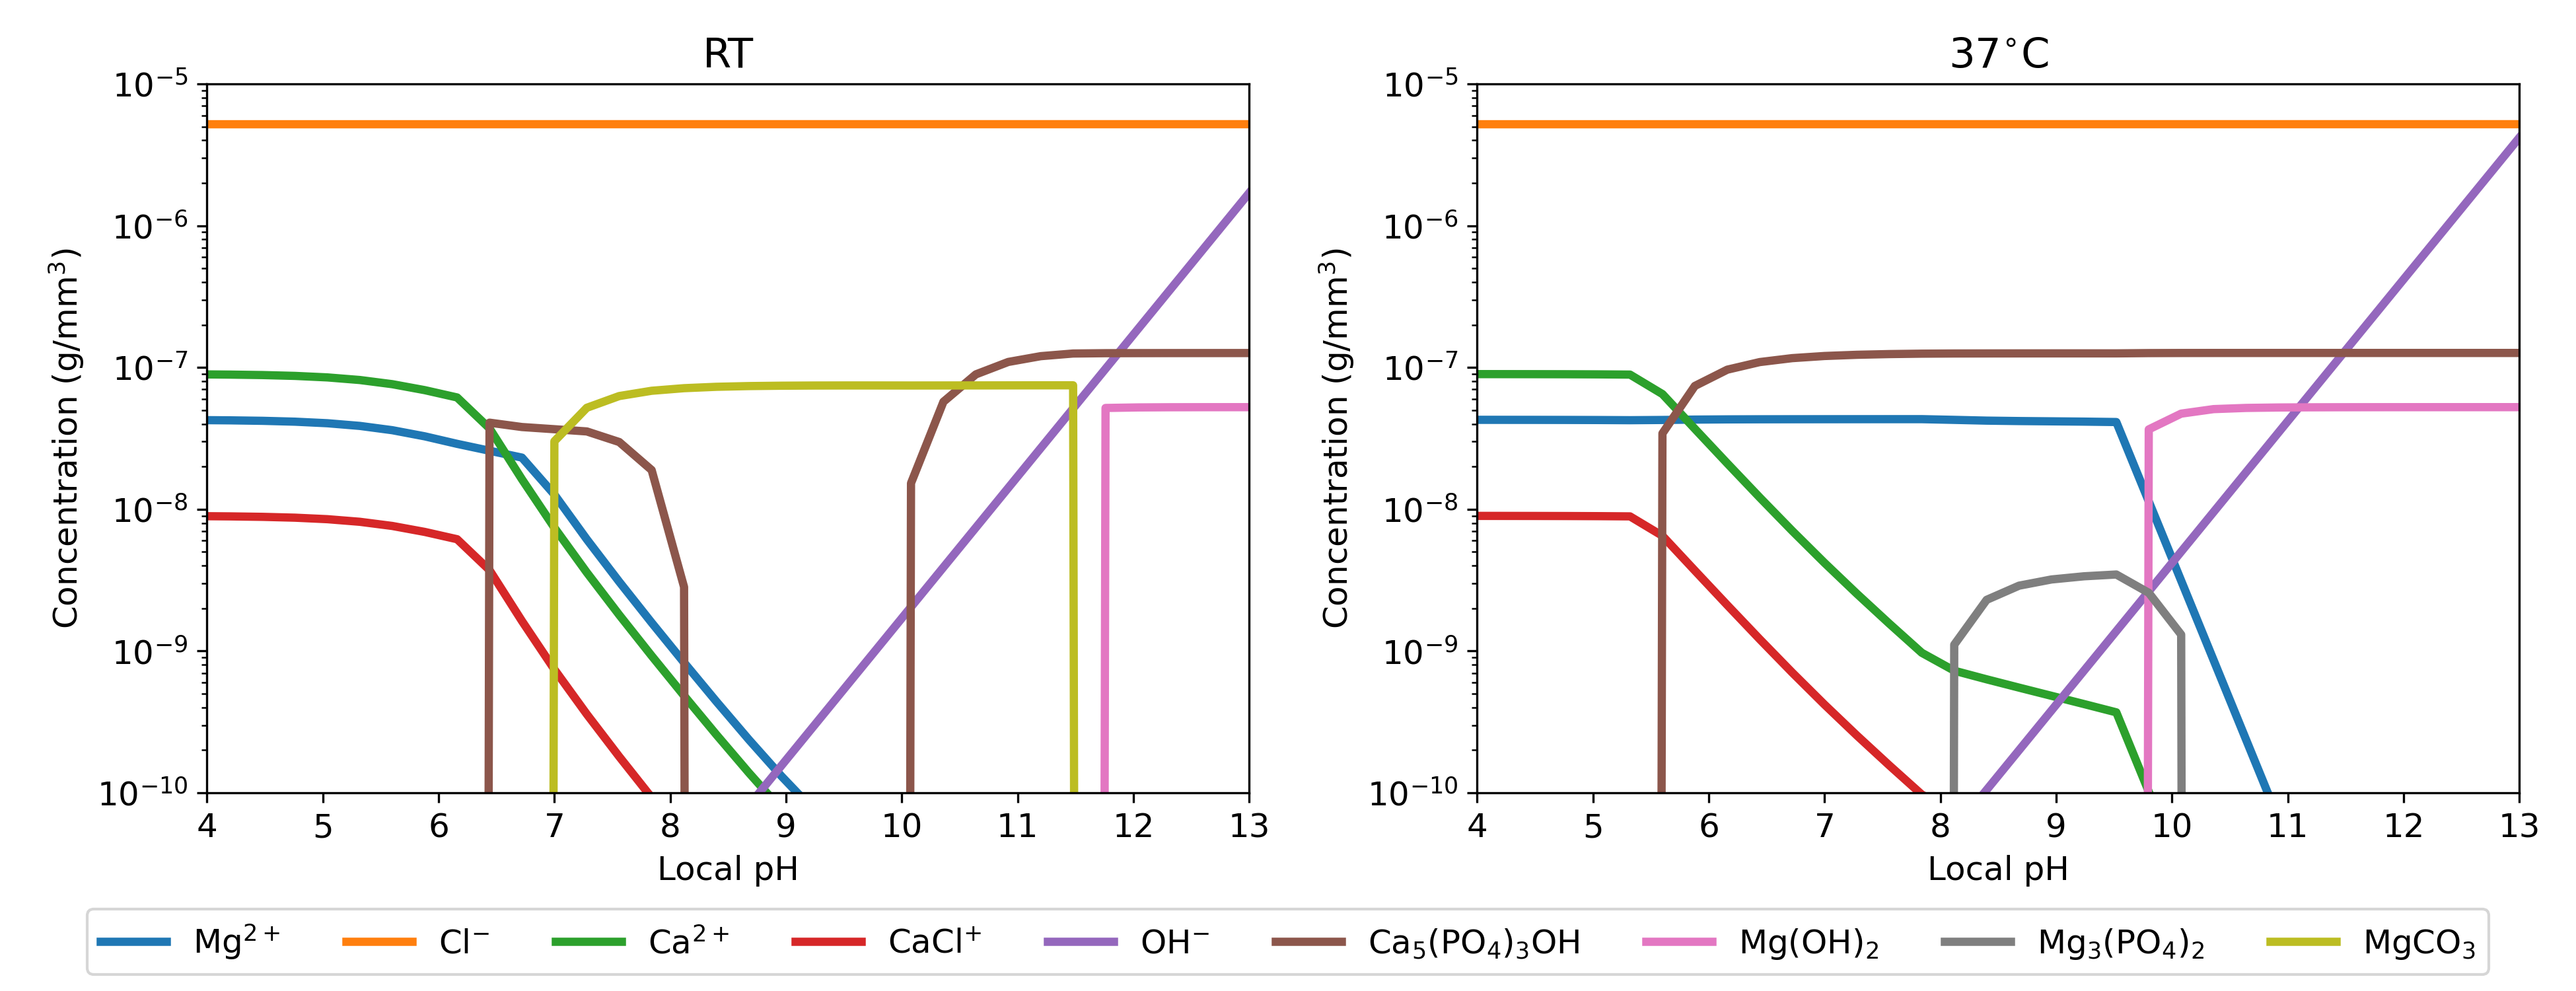
\includegraphics[width=\textwidth]{medusa_profiles.png}
\caption[Hydra-Medusa software output for given experiment conditions]{Selected components from the Hydra-Medusa software output for given experiment conditions} \label{fig:kinetics_medusa_profiles}
\end{figure}

\begin{figure}[h]
\centering
\medskip
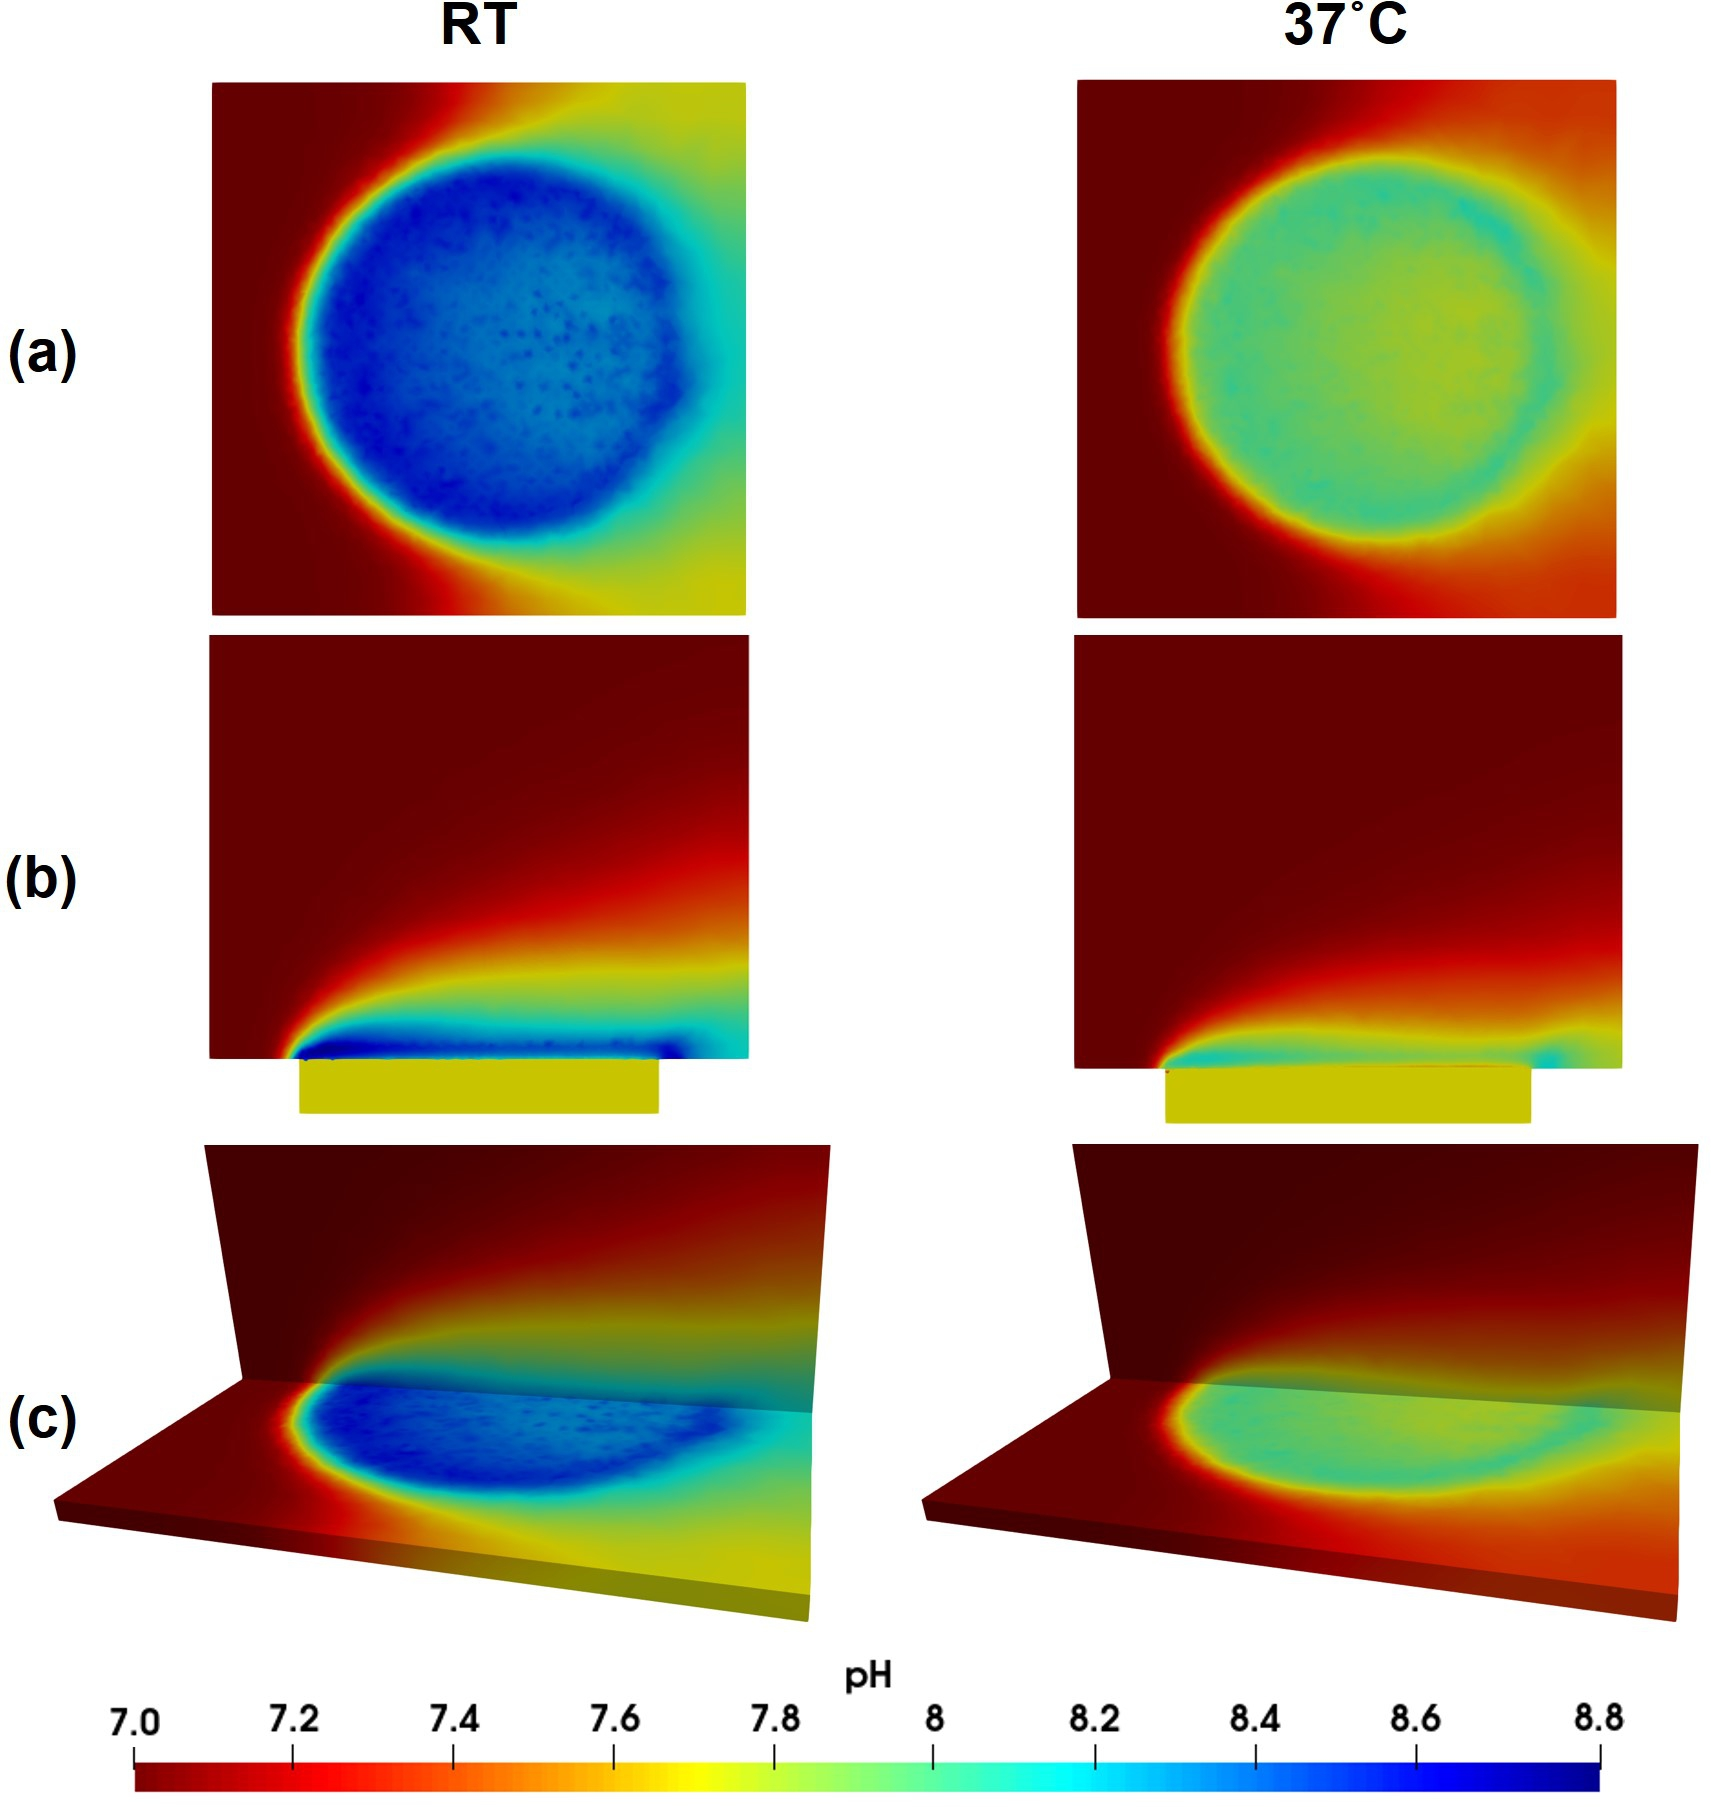
\includegraphics[width=\textwidth]{local_ph_visual.jpg}
\caption[Simulation results for local pH predictions]{Simulation results for local pH predictions} \label{fig:kinetics_local_ph_visual}
\end{figure}

\begin{figure}[h]
\centering
\medskip
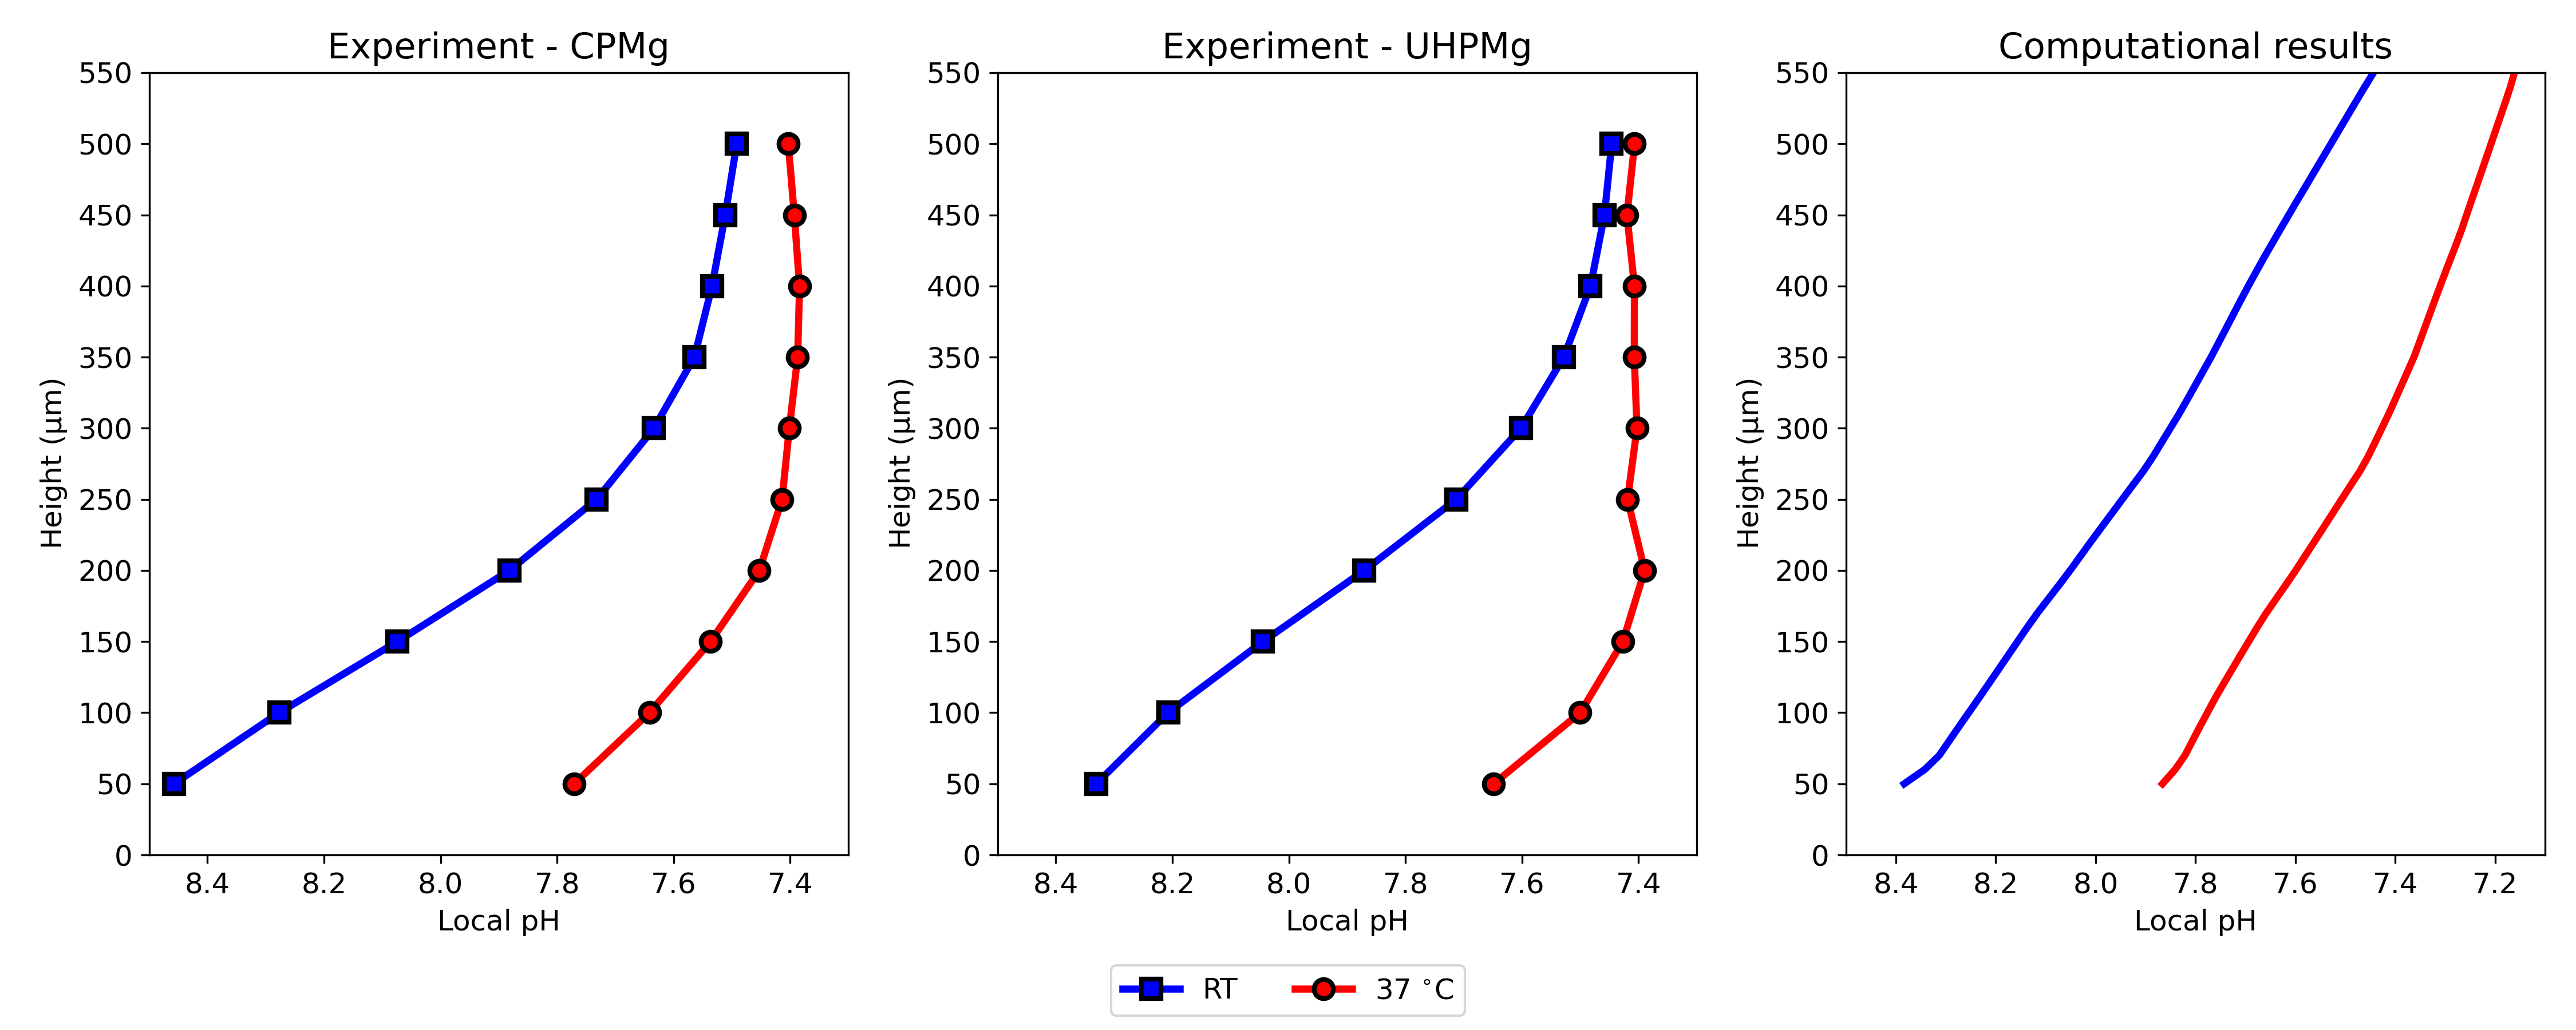
\includegraphics[width=\textwidth]{vertical_profile.png}
\caption[Comparing computational and experimental vertical pH profile]{Comparing computational and experimental vertical pH profile} \label{fig:kinetics_vertical_profile}
\end{figure}

\begin{figure}[h]
\centering
\medskip
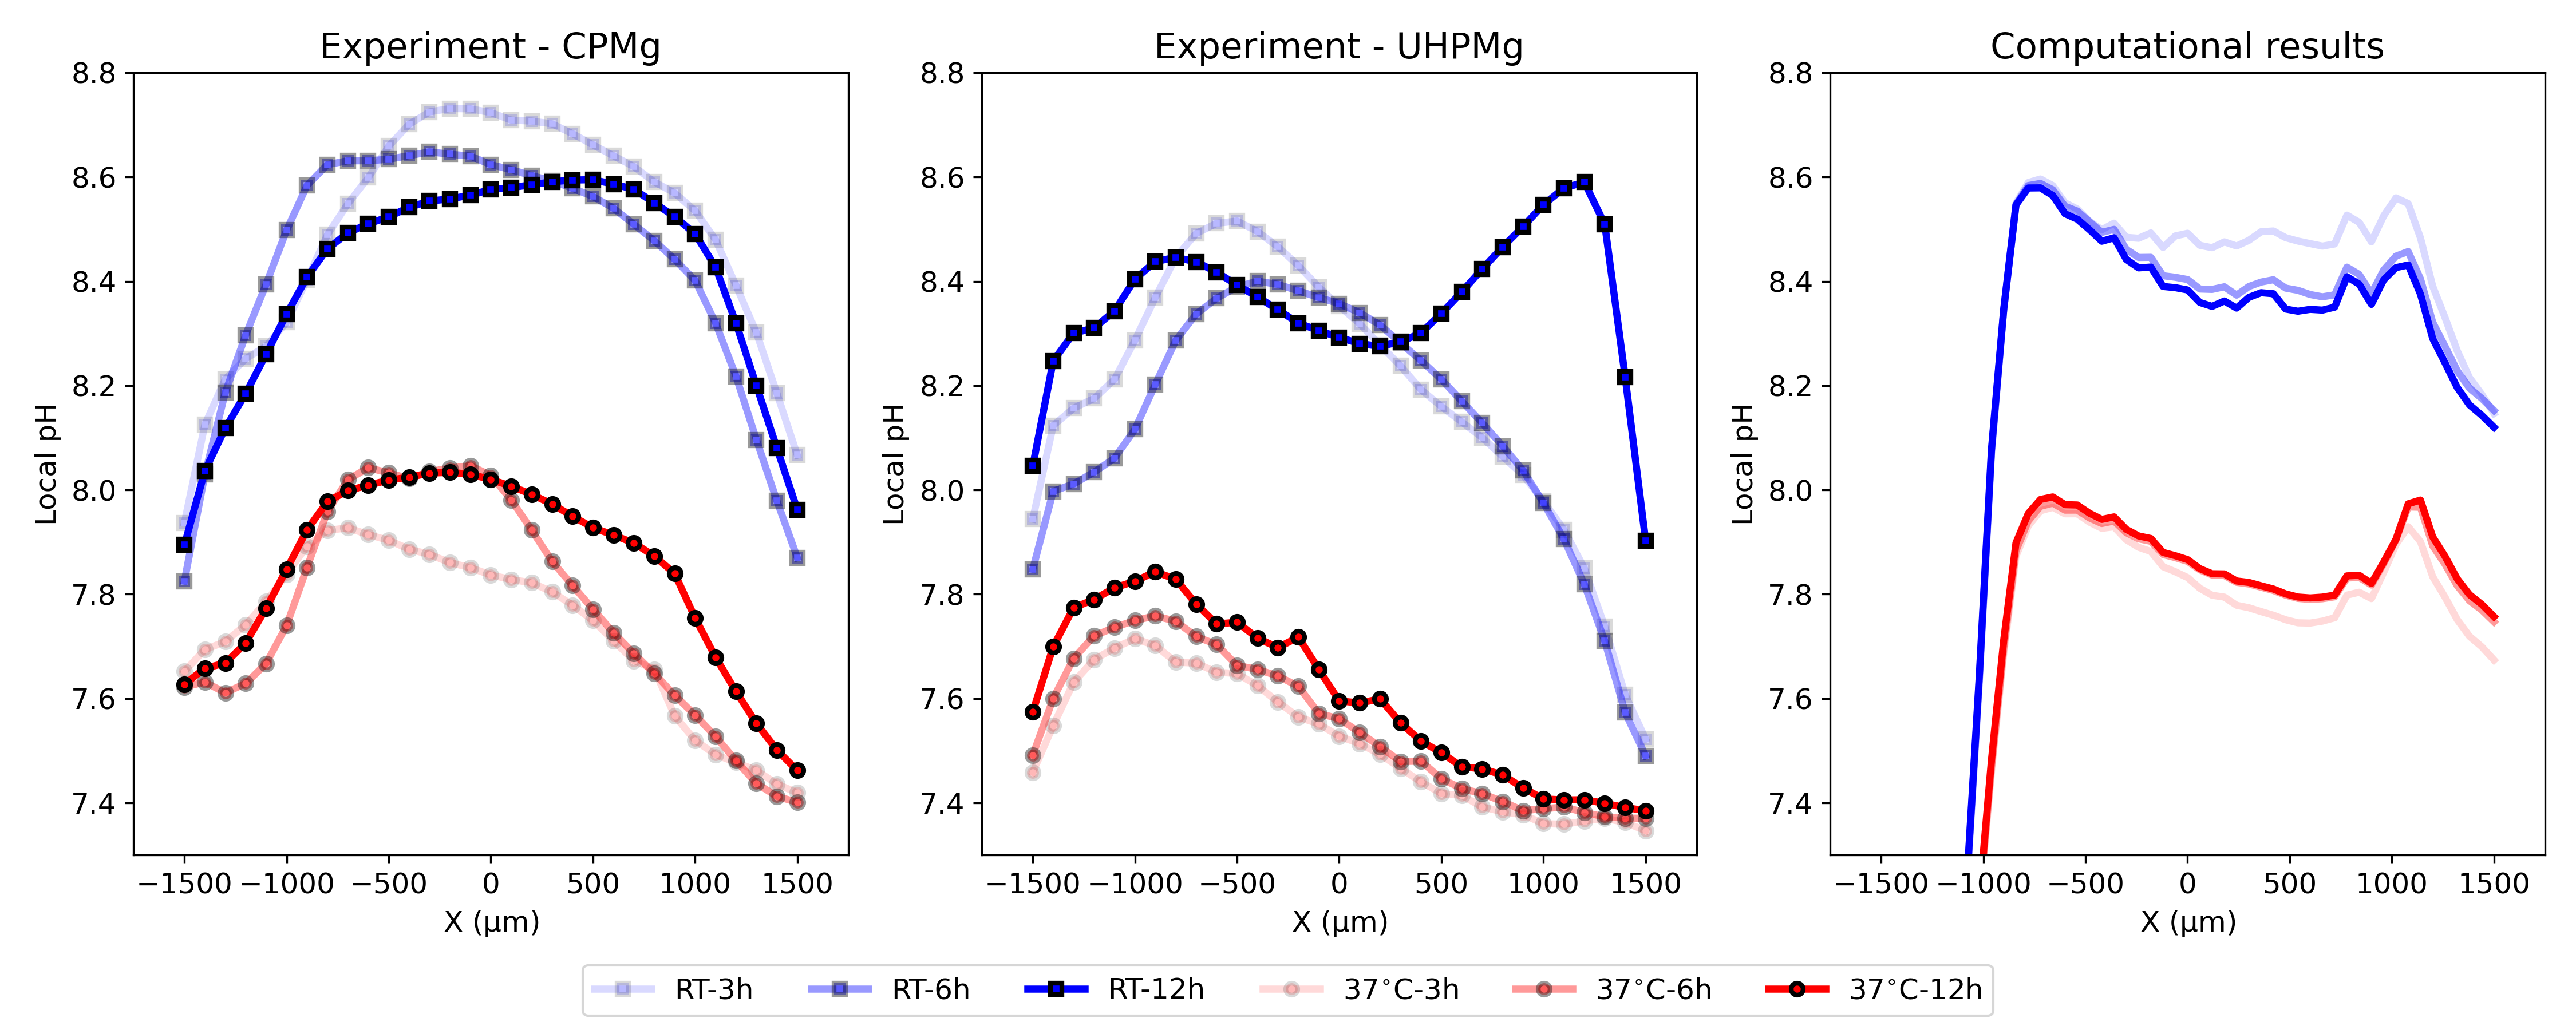
\includegraphics[width=\textwidth]{line_scans.png}
\caption[Comparing computational and experimental horizontal line scans for  local pH]{Comparing computational and experimental horizontal line scans for  local pH} \label{fig:kinetics_line_scans}
\end{figure}

\section{Discussion}

\section{Methods}

\begin{figure}[h]
\centering
\medskip
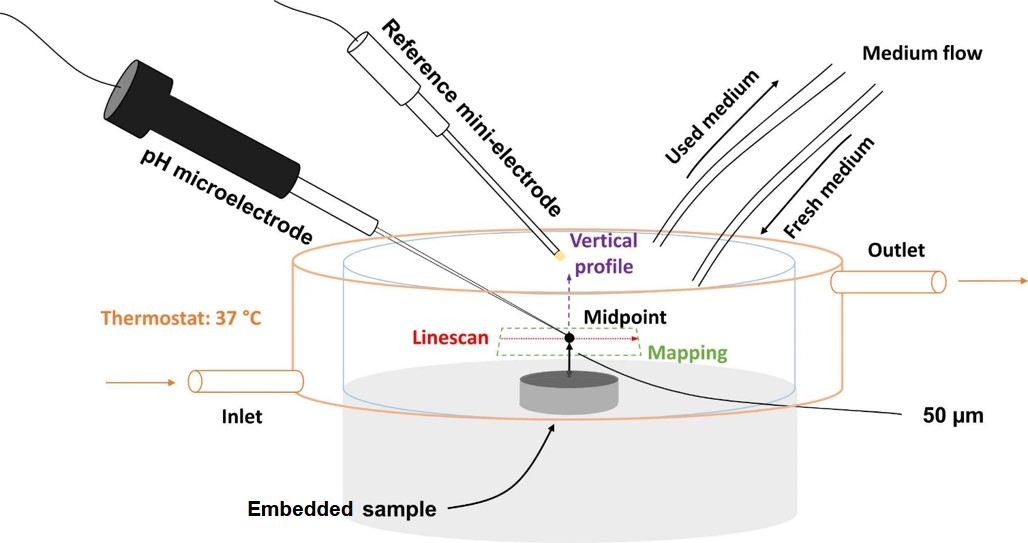
\includegraphics[width=0.8\textwidth]{setup.jpg}
\caption[Experimental setup for validating the coupled biodegradation model]{Experimental setup for validating the coupled biodegradation model} \label{fig:kinetics_setup}
\end{figure}


\begin{figure}[h]
\centering
\medskip
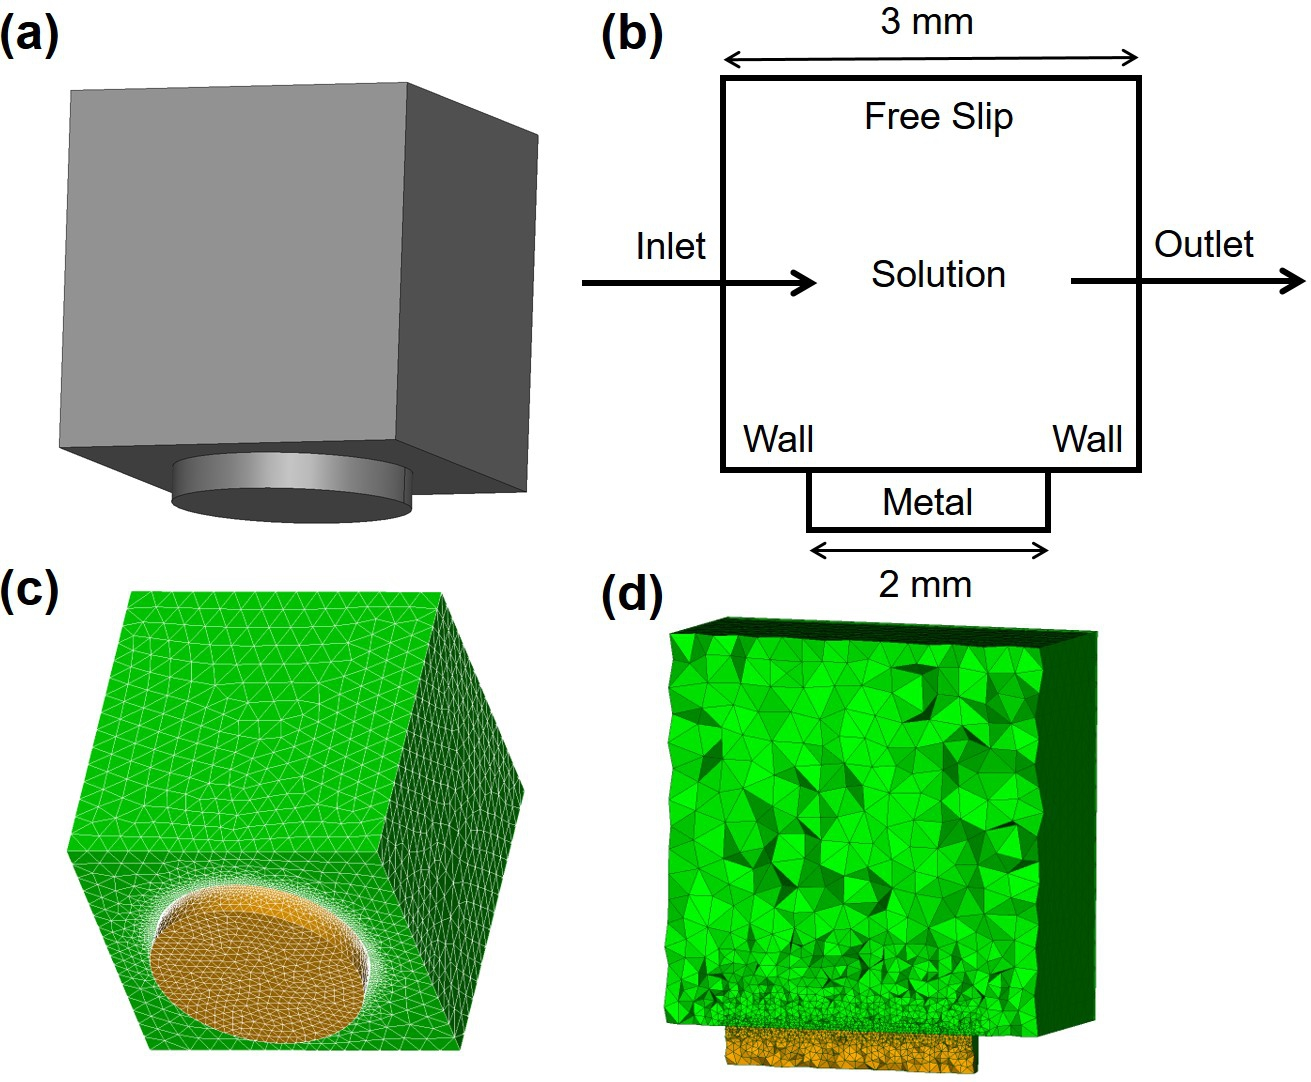
\includegraphics[width=\textwidth]{model_setup.jpg}
\caption[Computational model setup for local pH simulations]{Computational model setup for local pH simulations} \label{fig:kinetics_model_setup}
\end{figure}



\section{Data Availability}

The data used in the paper are available from the authors upon request.

\section{Code Availability}
The source code of the programs used in this paper is available from the authors upon request.


\section{Acknowledgements}

\section{Author Contributions}

\section{Competing Interests}


%%%%%%%%%%%%%%%%%%%%%%%%%%%%%%%%%%%%%%%%%%%%%%%%%%
% Keep the following \cleardoublepage at the end of this file, 
% otherwise \includeonly includes empty pages.
\cleardoublepage

